\subsection{Projekt oversigt}
I dette afsnit vises design, brugergrænseflade, implementering og test for 'ProjectList' viewet. For den fulde dokumentation henvises til Arkitektur og Design dokumentationens afsnit \ref{Design-sec:Opretbruger}.

\subsubsection{Design}
På Figur \ref{fig:ProjctListSekvens} ses sekvensdiagrammet for 'Project List' viewet til Rambøll Tilsyn.
\begin{figure}[H] % (alternativt [H])
	\centering
	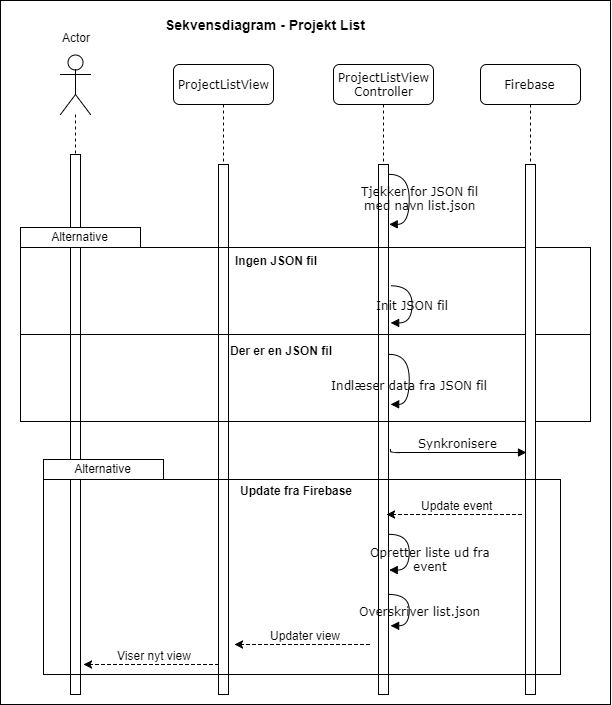
\includegraphics[height=15cm, width=12cm]{../ArkitekturDesign/Design/ProjectList/ProjektListSekvensDiagram}
	\caption{Sekvensdiagram for ProjectList i Rambøll Tilsyn.}
	\label{fig:ProjctListSekvens}
\end{figure}

\clearpage

\subsubsection{Grafisk brugergrænseflade}
I ProjectListViewet er der en oversigt over hvilke projekter der ligger i databasen, samt mulighed for tilføje projekt eller tilføj bruger. Se figur \ref{fig:ProjectListView}
\begin{figure}[H] % (alternativt [H])
	\centering
	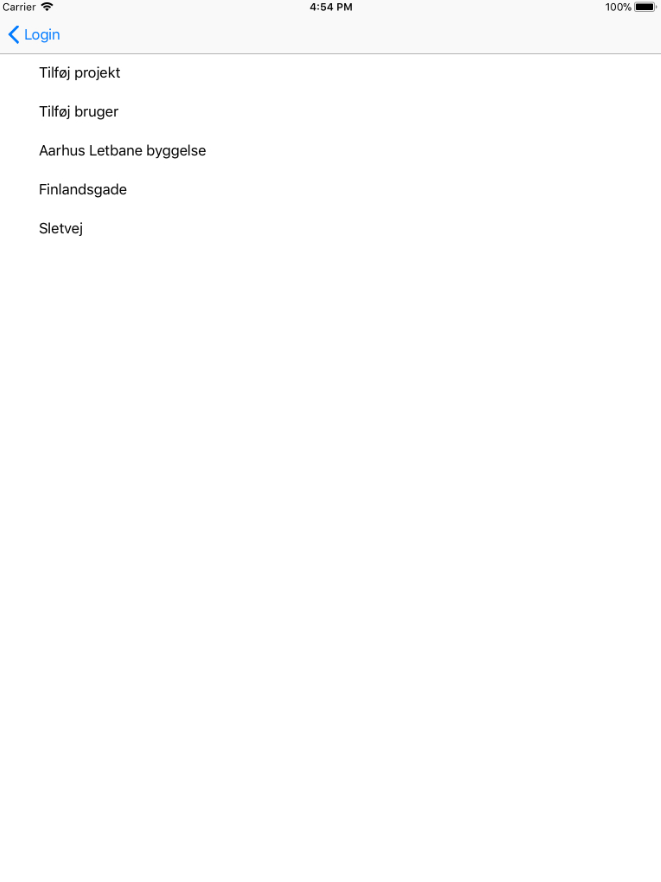
\includegraphics[height=12cm, width=10cm]{Design/Applikation/ProjektList/ProjectList}
	\caption{Project List viewet, som det er implementeret i Rambøll Tilsyn.}
	\label{fig:ProjectListView}
\end{figure}

\subsubsection{Implementering}
Før listen af projekter bliver vist for brugeren, initialiserer 'Project List' viewet en forbindelse til Firebase, hvor at den sætter et synkroniseringsevent, som kaldes såfremt der sker ændringer i PDF-filerne. \\
Dernæst opretter den en JSON-fil som indeholder alt projekt information fra Firebase. \\
Controlleren opretter nu et nyt TableView som har sourcen TableSource. Her laver den en liste bestående af alle projekter og muligheden for at tilføje bruger og tilføje projekt. \\
For en mere deltajeret beskrivelse af implementeringen og kode snips, henvises til Arkitektur og Design dokumentations afsnit \ref{Design-sec:ProjectList}.

\clearpage